\chapter{Grundlagen}
\label{cha:Grundlagen}
Im folgenden Kapitel sollen die zum Verständnis der Arbeit nötigen Grundlagen erläutert werden. Anfangs werden die elektrochemischen Grundlagen der Elektrolyse von Wasser vorgestellt sowie deren thermodynamische Zusammenhänge geschildert. Zudem wird die ideale Zellspannung hergeleitet und es werden wesentliche Verlustmechanismen sowie deren Einfluss auf den Betriebsbereich von Elektrolyseuren benannt. Weiterhin werden gängigen technischen Lösungen der Wasserelektrolyse vorgestellt. Im Anschluss werden Gemeinsamkeiten und Unterschiede von Elektrolyseuren und Brennstoffzellen dargelegt. \\


\section{Grundlagen der Wasserelektrolyse}
\label{sec:Elektrolyse}
Als Elektrolyse bezeichnet man einen chemischen Prozess, bei dem eine Redoxreaktion durch elektrische Spannung erzwungen wird. 
Um eine kontrollierbare Durchführung der Reaktion sicherzustellen, ist eine räumliche und elektrische Trennung der Oxidation und Reduktion nötig \citep{tjarks_pem-elektrolyse-systeme_2017}. Allerdings muss der Ionenaustausch zwischen Anode und Kathode möglich sein und dies wird durch ein Elektrolyt erreicht.\\

Bei der Wasserelektrolyse wird dieses Prinzip angewendet, um aus Wassermolekülen elementaren Wasserstoff und Sauerstoff zu gewinnen. Dabei liegt folgende allgemeine Reaktionsgleichung vor:   
\begin{align}
	\label{gl:Reaktionsgleichung}
	\ce{ H2O &-> H2 + 1/2O2}
\end{align}
Die allgemeine Reaktionsgleichung ist dabei unabhängig vom Elektrolyt, wohingegen sich die Oxidations- und Reduktionsgleichungen unterscheiden. Die Oxidation findet an der Anode statt und hat Sauerstoff als Produkt. An der Kathode wird durch die Reduktion Wasserstoff gebildet. Es gibt drei mögliche Ladungsträger bei der Wasserelektrolyse: Hydroxidionen, Protonen oder Oxidionen \citep{tjarks_pem-elektrolyse-systeme_2017}. Zu den verschiedenen Ladungsträgern werden in  \ref{par:Alkalischer Elektrolyseur} bis \ref{par:Feststoffoxid Elektrolyseur} technische Verfahren angeführt und erläutert.\\

\begin{figure}[h]
	\centering
		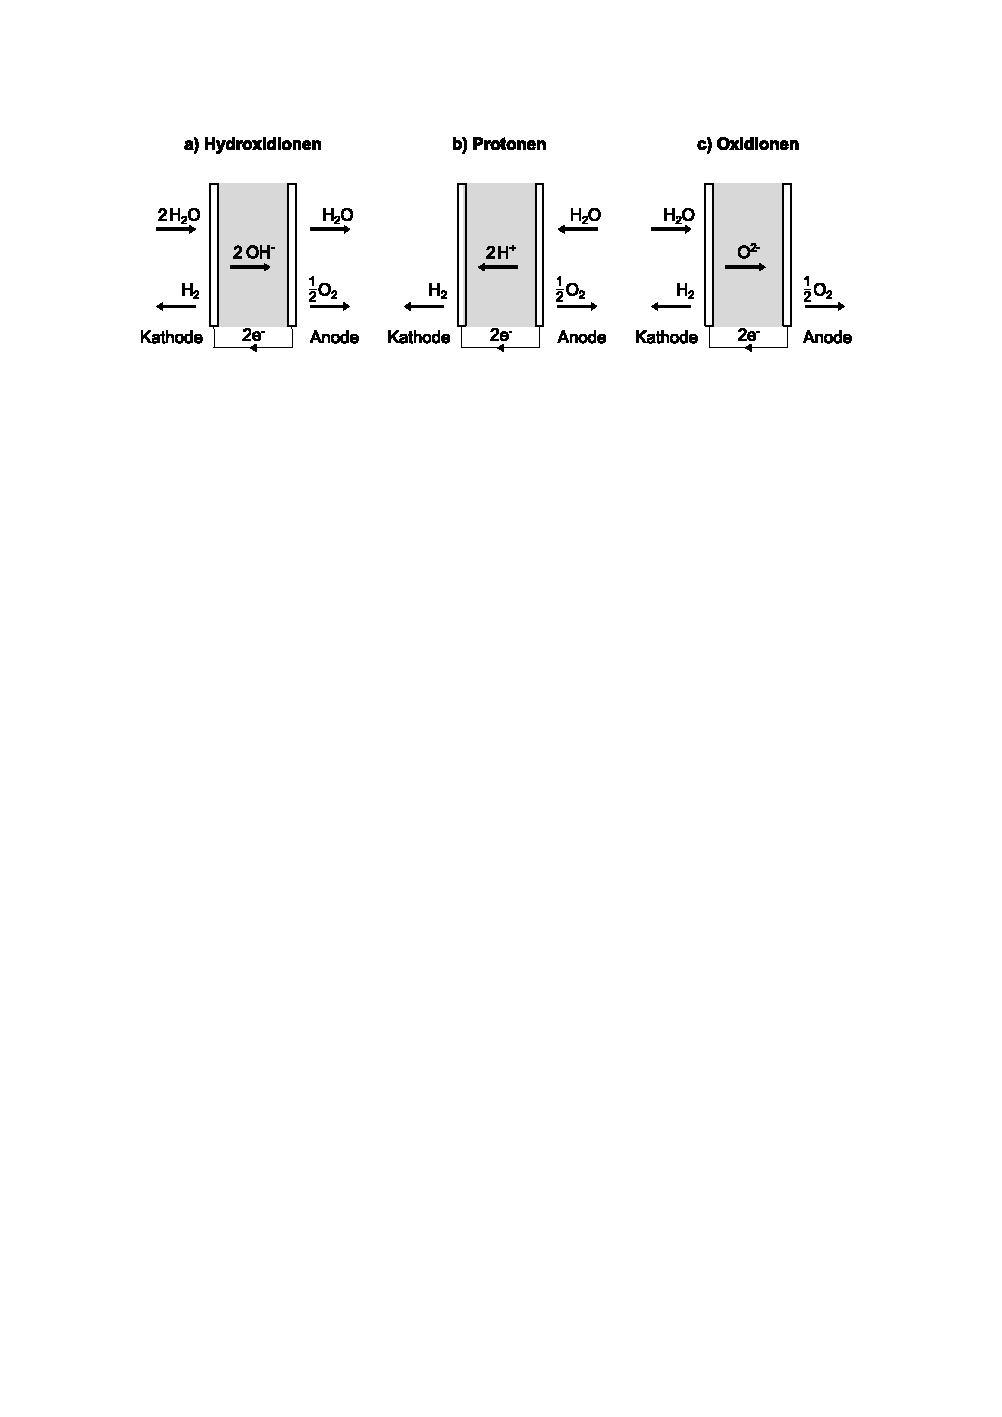
\includegraphics[scale=1]{Figures/LadungstraegerBeiDerWasserelektrolyse}
		\caption{Ladungsträger bei der 
		Wasserelektrolyse \citep{tjarks_pem-elektrolyse-systeme_2017}}
\label{fig:LadungstraegerBeiDerWasserelektrolyse}	
\end{figure}

\subsection{Elektrochemische Betrachtung}
\label{subsec:Energetische Betrachtung}
Die benötigte Energie bei einer Redoxreaktion entspricht der Reaktionsenthalpie $\Delta H_R$ und lässt sich aus den Bildungsenthalpien ($\Delta_f H_i$) und stöchometrischen Koeffizienten ($\nu_i$) der Edukte und Produkte bestimmen \citep{falcao_review_2020,brauns_alkaline_2020}:
\begin{align}
 	\Delta H_R = \sum{\nu_i \Delta_f H_i}
\end{align}
Unter der Annahme, dass die nötige thermische Energie vorliegt, entspricht die zur Reaktion benötigte elektrische Energie  der freien Reaktionsenthalpie $\Delta G_R$, welche sich über die Reaktionsentropie $\Delta S_R$ errechnen lässt.
\begin{align}
	\Delta G_R = \Delta H_R - T\Delta S_R \\
 	\Delta S_R = \sum{\nu_i S_i}
\end{align}

Für die Wasserelektrolyse (\ref{gl:Reaktionsgleichung}) bei Standardtbedingungen ($T_0 = \SI{25}{\degreeCelsius}$ und $p_0 = \SI{101,325}{\kilo\pascal}$) ergibt sich mit den Daten aus Tabelle \ref{tb:Stoffdaten} die Reaktionsenthalpie zu $\Delta H^0_R = \SI{285,25}{\kilo\J\per\mol}$ und die freie Enthalpie zu $\Delta G^0_R = \SI{236,59}{\kilo\J\per\mol}$.\\ 
h-700 = 247,12; g-700 = 193,66
\begin{table}[ht]
		\centering
		\caption{Standardtbildungsenthalpien und Standardtentropien für $\SI{25}{\degreeCelsius}$ \citep{koj_entwicklung_2021} und $\SI{700}{\degreeCelsius}$ \citep{Informatics} sowie stöchometrische Koeffizienten aus \ref{gl:Reaktionsgleichung}}
		\begin{tabular}{c c c c c c}
		\toprule
		\multirow{2}{*}{Komponenten i} & 
		\multicolumn{1}{c}{$\Delta_f H^0_i$} & 
		\multicolumn{1}{c}{$\Delta_f H_i (T=\SI{700}{\degreeCelsius})$} &
		\multicolumn{1}{c}{$S^0_i$} &
		\multicolumn{1}{c}{$S_i (T=\SI{700}{\degreeCelsius})$} &
		\multicolumn{1}{c}{$\nu_i$}
		\\
		& 
		\multicolumn{1}{c}{$\textrm{[kJ/mol]}$}& 
		\multicolumn{1}{c}{$\textrm{[kJ/mol]}$}& 
		\multicolumn{1}{c}{$\textrm{[J/(molK)]}$} &
		\multicolumn{1}{c}{$\textrm{[J/(molK)]}$} &
		\multicolumn{1}{c}{$\textrm{[--]}$}
		\\
		\midrule
		$\ce{H2O}$ & -285,25 & 70,12 & -216.35 & 231,81 & -1\\
		$\ce{O2}$ & 0 & 205,25 & 21,78 & 242,64 & $\textrm{1/2}$\\
		$\ce{H2}$ & 0 & 130,7 & 19,88 & 165,43 & 1\\
		\bottomrule
		\end{tabular}
		\label{tb:Stoffdaten}
		\end{table}	
			
\paragraph{Reversible Zellspannung}
\label{par:rev Zellspannung}
Mit der Faraday Konstante ($F=\SI{96485,3}{\coulomb\per\mol}$) und der Anzahl der pro Reaktion transferierten Elektronen ($z = 2$) lässt sich die thermoneutrale Spannung bei Standardtbedingungen $U^0_{tn}$ sowie die reversible Zellspannung bei Standardbedingungen $U^0_{rev}$ errechnen \citep{falcao_review_2020}. 

\begin{align}
 U^0_{tn} = \frac{\Delta H^0_R}{zF} = \SI{1,478}{\volt}\\
 U^0_{rev} = \frac{\Delta G^0_R}{zF} = \SI{1,226}{\volt}
\end{align}

Dabei ist zu beachten, dass sowohl die Reaktionsenthalpie als auch die freie Enthalpie eine starke Temperaturabhängigkeit aufweisen, was sich auch auf die Spannungen auswirkt (\ref{fig:Entropien}).

\begin{figure}[h]
	\centering
		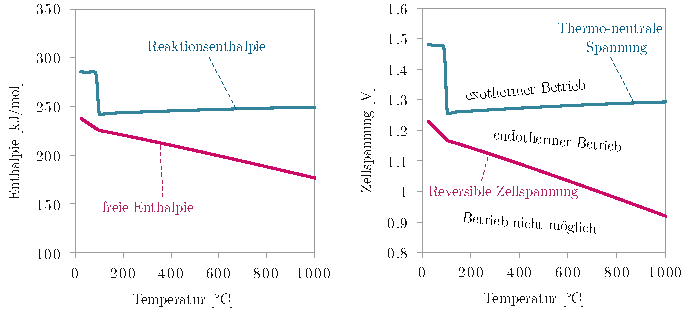
\includegraphics[scale=1]{Figures/VerlaufVonEntropien}
		\caption{Abhängigkeit der Reaktionsenthalpie und der freien Enthalpie von der Temperatur nach \citet{tremel_electrolysisfundamental_2018}}
\label{fig:Entropien}	
\end{figure}

\subsubsection{Überspannungen}
\label{subsubsec:Überspannungen}
Die reale Zell-Spannung $U_{real}$ ist im Betrieb aufgrund von Verlusten immer größer als die reversiblen Zellspannung. Ist die reale Zellspannung niedriger, als die thermoneutrale Spannung, läuft das System endotherm ab. In dem Fall muss dem System Wärmeenergie zugeführt werden. Nach \citet{olivier_low-temperature_2017} ist die Zellspannung im realen Betrieb aufgrund der Verluste stets größer als die thermoneutrale Spannung, das System wird also exotherm betrieben und es muss Wärmeenergie abgeführt werden (\ref{fig:Entropien}).\\
Als maßgeblichen Verluste, auch Überspannungen genannt, werden üblicherweise drei Phänomene betrachtet: Aktivierungsverluste ($U_{Akt}$), Ohmsche Verluste ($U_{Ohm}$) und Konzentrationsüberspannung ($U_{Diff}$)\citep{falcao_review_2020}. Ein weiteres Phänomen sind Diffusionsströme von Wasserstoff auf die Anodenseite und von Sauerstoff auf die Kathodenseite, allerdings sind diese aus Sicherheitsaspekten gering zuhalten, was in \ref{subsec:Polarisationskurve} näher erläutert wird. Daher werden Diffusionsströme in dieser Arbeit als vernachlässigbar klein angenommen. 
\begin{align}
	\label{gl:U_real}
	U_{real} =  U_{rev} + U_{Akt} + U_{Ohm} + U_{Diff}
\end{align}   
\paragraph{Aktivierungsverluste} \ \\
Aktivierungsverluste kommen durch die elektrochemischen Vorgänge an den Oberflächen er Elektroden und ihrer Kinetik zustande. Dabei treten zwei Phänomene auf:  Einerseits chemische (wegen des chemischen Gleichgewichtszustands der Ionen an der Grenzfläche zwischen Elektrode und Elektrolyt) und andererseits elektrische (aufgrund des Ladungstransports durch das elektrische Feld an der Grenzfläche)\citep{stempien_solid_2013}.\\

\paragraph{Ohmsche Verluste} \ \\
Ohmsche Verluste werden durch elektrische sowie ionische Widerstände und Kontaktwiderständen zwischen den Komponenten verursacht. Ionischen Widerstände, welche sich in der Membran (bei alkalischer und PEM-Elektrolyse) und an den Elektrodenoberflächen lokalisieren lassen, dominieren üblicherweise die Ohmschen Verluste \cite{stempien_solid_2013}. Elektrisch Widerstände treten in den Elektroden und an der Kontaktierung der Zelle auf und lassen sich somit durch den Aufbau der Zelle beeinflussen \citep{tjarks_pem-elektrolyse-systeme_2017}.\\

\paragraph{Diffusionsüberspannungen}\ \\
Diffusionsüberspannungen treten auf, wenn eine Überpopulation von Produktgasen an den Elektroden entsteht. Die Gase bilden Blasen auf den Elektrodenoberflächen und verringern dadurch die Fläche, an welcher die Teilreaktionen stattfinden können \citep{abdin_modelling_2015}. Diffusionsüberspannungen treten somit verstärkt bei hohen Stromdichten auf und bewirken daher ein sinkenden Wirkungsgrad bei steigender Stromdichte \citep{biaku_semiempirical_2008}.\\

\subsection{Polarisationskurve und Betriebsbereiche von Elektrolyseuren}
\label{subsec:Polarisationskurve}
Die Abhängigkeit der realen Zellspannung $U_{real}$ eines Elektrolyseurs von der Stromdichte bildet die Polarisationskurve graphisch ab. Diese wird von vielen Einflussfaktoren - wie beispielsweise den Elektrodenmaterialien, der Geometrie der einzelnen Bauteile oder den Betriebsbedingungen wie Druck und Temperatur - beeinflusst. \textbf{Grundlage für die Berechnung der Polarisationskurve ist die in \ref{subsec:rev Zellspannung} hergeleitete reversible Zellspannung und Gleichung \ref{gl:U_real}.} \ref{fig:PolarisationskurveElektrolyseure} vergleicht die Polarisationskurven der in \ref{subsec:Gängige Technologien der Wasserelektrolyse} erläuterten technischen Verfahren. 
\begin{figure}[h]
	\centering
		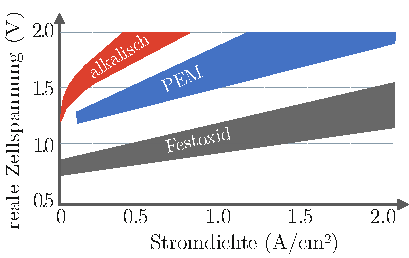
\includegraphics[scale=1]{Figures/PolarisationskurvenElektrolyseure}
		\caption{Mögliche Bereiche der Polarisationskurven verschiedener Elektrolyse-Technologien nach \citet{tremel_electrolysisfundamental_2018}}
\label{fig:PolarisationskurveElektrolyseure}	
\end{figure}

Des weiteren lässt sich die Polarisationskurve auch zur Bestimmung des Betriebspunkts nutzen:\\
Die elektrische Leistung einer Zelle ($P_el$) lässt sich aus der Stromdichte ($i$), der aktiven Fläche ($A_zelle$) und der realen Zellspannung errechnen. Das Faradaysche Gesetz liefert einen direkten Zusammenhang zwischen de Elektronenfluss und dem Stoffmenge an produziertem Wasserstoff ($\dot{n}_{H_2O}$).
\begin{align}
	P_{el}(i) = U_{real}(i)\cdot i A_{zelle}\\
	\dot{n}_{H_2O} = \frac{i A_{zelle}}{zF}
\end{align}
Der Wirkungsgrad ($\eta$) einer Zelle, bezogen auf den unteren Heizwert ($H_u$) von Wasserstoff wird damit durch folgenden Ausdruck beschrieben:
\begin{align}
	\eta = \frac{H_u \cdot\dot{n}_{H_2O}}{P_{el}} = \frac{H_u}{U_{real}(i)\cdot{zF}}
\end{align}
Somit zeigt sich, dass es zur Steigerung der Effizienz erstrebenswert ist, den Elektrolyseur bei einer niedrigen Spannungen zu betreiben \citep{biaku_semiempirical_2008}. Aus \ref{fig:PolarisationskurveElektrolyseure} wird ersichtlich, dass dies bei einer niedrigen Stromdichte der Fall ist. Allerdings bleibt zu bedenken, dass dadurch auch der Produktgasstrom verringert wird, weshalb ein Kompromiss zwischen Wirkungsgrad und einer größeren aktive Zellfläche - und damit verbunden höheren Investitionskosten und größerem Bauraum - zu finden ist.\\
Weiterhin stellt die Gasreinheit der Produktströme eine untere Betriebsgrenze für die Stromdichte dar. Aufgrund von Diffusion der Produktgase durch die Membran (bei Alkalischer und PEM-Elektrolyse) bzw. das Elektrolyt(bei SO-Elektrolyse), kommt es zu einer Mischung von Sauerstoff und Wasserstoff. Da beide Produktgase ab einer Verunreinigung von $4$ Volumen-\% explosive Mischungen bilden können, wird üblicherweise bei 2 Volumen-\% Verunreinigung ein Notstop des gesamten Elektrolyseur-Systems eingeleitet \cite{brauns_alkaline_2020}. Zwei physikalische  Abhängigkeiten sind dabei bedeutsam:\\ 
Einerseits nimmt die Verunreinigung der Produktgase bei hohem Druck zu, da dann auch der für die Diffusion maßgebliche Konzentrationsgradient eines Gases in der Membran/dem Elektrolyt steigt.
Andererseits sinkt die Verunreinigung bei steigender Stromstärke, weil die produzierte Stoffmenge mit der Stromdichte linear ansteigt, der Diffusionsstrom aber wegen gleichbleibender Konzentrationsverläufe  nahezu konstant ist. Somit wird die Verunreinigung bei einer höheren Stromdichte stärker verdünnt \citep{brauns_alkaline_2020}.\\
\citet{grigoriev_high-pressure_2011} gibt an, dass die Verunreinigung der Produktgase insbesondere durch die Rekombination von Wasserstoff und Sauerstoff verringert werden kann.  Somit kann durch bestimmte Maßnahmen der Betriebsbereich in Richtung niedrigerer Stromstärken vergrößert werden.

\subsection{Technologien der Wasserelektrolyse}
\label{subsec:Technologien der Wasserelektrolyse}
\textbf{Im folgenden sollen die drei maßgeblichen Verfahren zur Wasserelektrolyse näher erläutert werden.}
\paragraph{Alkalischer Elektrolyseur}
\label{par:Alkalischer Elektrolyseur}
Die alkalische Elektrolyse ist eine ausgereifte Technik und der derzeitige Standard für groß dimensionierte Elektrolyseure \citep{tremel_electrolysisfundamental_2018}. Anlagen mit einer Leistung Wasserstoffproduktion von bis zu \SI{130}{\mega\W}  sind derzeit im Betrieb und die minimale Teillast liegt nach \citep{guandalini_comparative_2016} bei ungefähr 20\%. Als Elektrolyt dient üblicherweise zwischen 25 und 30 prozentige Natron- (NaOH) oder Kalilauge (KOH) \citep{tremel_electrolysisfundamental_2018}. Grund für die hohe Konzentration ist, dass der Base-Gehalt der Lösung maßgeblich deren Leitfähigkeit beeinflusst. Als Ladungsträger in der Lösung fungieren Hydroxidionen. Es werden metallische Elektroden verwendet, welche gelegentlich zur Steigerung der Aktivität mit Edelmetallen beschichtet werden. Folgende Reaktionen laufen an der Kathode und Anode ab:
\begin{align}
  \ce{	&{Kathode:} &2H2O + 2 e^- &-> H2 + 2OH^-\\
  		&{Anode:} &2OH^- &-> H2O + O2 + 2 e^-} 
\end{align}
Um die produzierten Gase von einander getrennt zu halten, wird zwischen Anode und Kathode ein Diaphragma positioniert. Dies hat neben Performance- auch Sicherheitsgründe, da elementarer Wasserstoff hochentzündlich ist. Aus diesem Grund sind Elektrolyseure auch in ihrer Dynamik eingeschränkt: Bevor das System abgeschaltet werden kann, müssen die Gasleitungen mit Inertgas gefüllt werden, um die Bildung einer explosiven Wasserstoff-Sauerstoff Mischung zu verhindern. Dies hat auch einen Einfluss auf den Anlaufvorgang des Systems, da die Gasqualität durch die anfangs vorliegenden Inertgase vermindert wird. Nach \citet{Milanzi} kann das dynamische Verhalten von Elektrolyseuren erheblich verbessert werden, wenn sie wärend Standzeiten im Standby betrieben werden. \\ 
Ein weiterer Nachteil aktueller technischer Anlagen der alkalischen Elektrolyse ist, das die maximale Stromdichte verglichen mit anderen Elektrolyseuren niedrig ausfällt (\citet{tremel_electrolysisfundamental_2018} gibt Stromdichten von $0,2-\SI{0,5}{\A\per\cm\squared}$ an).

\paragraph{Protonen Austausch Membran (PEM) Elektrolyseur}
\label{par:Protonen Austausch Membran (PEM) Elektrolyseur}
PEM-Elektrolyseure werden seid 1950 entwickelt und derzeit im $\SI{1}{\mega\W}$ Bereich vertrieben. Ein Vorteile der Technologie sind die hohen erreichbaren Stromdichten von bis zu $\SI{0,5}{\A\per\cm\squared}$. Zudem können PEM-Elektrolyseure sehr dynamisch betrieben werden und ein Betrieb bei bis zu 10\% minimaler Teillast ist möglich \citep{tremel_electrolysisfundamental_2018}.\\
Als Ladungsträger fungieren Protonen und als Elektrolyt dient eine in destilliertem Wasser positionierte Protonen-Austausch-Membran (\textbf{P}roton \textbf{E}xchange \textbf{M}embran). Dies vereinfacht den Betrieb verglichen mit den mit stark basischer Lösung befüllten, alkalischen Elektrolyseuren erheblich. Die Protonenleitfähigkeit der Polymer-Membran wird durch Sulfonsäure-bindende Seitengruppen, sogenannte Idomere, erreicht \citep{tjarks_pem-elektrolyse-systeme_2017}.  Für die Dicke der Membran muss dabei ein Kompromiss zwischen Langlebigkeit und Durchlässigkeit gefunden werden \citep{falcao_review_2020}. Die Säure des Elektrolyts, so wie das Erstreben hoher Reaktionsgeschwindigkeiten führt zu hohen Kosten bei den Elektrodenmaterialien: Die Kathode besteht meist aus mit Platin beschichtetem Kohlenstoff, als Anode werden häufig als Oxid vorliegendes Irdium oder Ruthenium verwendet. Folgende Reaktionen laufen an der Kathode und Anode ab:
\begin{align}
  \ce{	&{Kathode:} &2H^+ + 2e^- &-> H2\\
  		&{Anode:} &H2O  &->  1/2O2 + 2H^+ + 2 e^-}
\end{align}
  		
\paragraph{Feststoffoxid Elektrolyseur}
\label{par:Feststoffoxid Elektrolyseur}
Feststoffoxid(SO) Elektrolyseure sind seid 1980 in Entwicklung \citep{isenberg_energy_1981} ? hier besser Übersicht angeben?. Sie haben  den Vorteil, dass sie Temperaturen von $700-\SI{1000}{\degreeCelsius}$ betrieben werden, wodurch dampfförmiges Wasser zerlegt wird, wohingegen bei alkalischen und PEM-Elektrolyseuren flüssiges Wasser vorliegt. Daraus resultiert, dass Reaktionsenthalpie und dadurch auch die reale Zellspannung niedriger ausfällt. Dieser Effekt wird dadurch verstärkt, dass bei hohen Temperaturen die ohmschen Verluste sinken, wodurch niedrigere Überspannungen entstehen \citep{tremel_electrolysisfundamental_2018}. Zudem steigt mit der Temperatur auch die Reaktionsgeschwindigkeit, weshalb keine teuren Katalysator-Materialien verwendet werden müssen \citep{yan_performance_2017}.\\
Ein Nachteil der gesteigerten Betriebstemperatur sind die höheren Ansprüche an die Temperaturbeständigkeit der Elektroden und des Elektrolyts. Als Elektrolyt wird meist Zirconiumdioxid ($\ce{ZrO2}$) verwendet, welches zur Steigerung Leitfähigkeit mit Yttriumoxid ($\ce{Y2O3}$) stabilisiert wird \citep{butz_decomposition_2009}.
Das Elektrolyt wird zwischen zwei porösen Elektroden (Beispielsweise eine Nickeloxid Anode und eine LSCF-Kathode \citep{schiller_high_2010}) positioniert, was den Austausch der Oxidionen ermöglicht. Es existieren SO-Elektrolyseure, welche auf dem Transport von Protonen basieren, allerdings soll aufgrund ihrer geringen Bedeutung  in dieser Arbeit nicht weiter darauf eingegangen werden \citep{stempien_solid_2013}.
\begin{align}
  \ce{	&{Kathode:} &H2O &-> H2 + O^2- + 2e^-\\
  		&{Anode:} &O^2- + 2 e^-  &->  1/2O2} 
\end{align}
Eine Herausforderung ist das Bereitstellen der benötigten Wärme zur Wasserdampferzeugung und zum Aufrechterhalten der Betriebstemperatur. Dazu werden verschiedene Möglichkeiten, wie beispielsweise die Kopplung mit Wärmepumpen oder Sonnenkollektoren in Betracht gezogen \citep{stempien_solid_2013}. Weiterhin bleibt ein zu lösendes Problem der Leistungsverlust und der Abbau der Elektrodenmaterialien, was die Lebensdauer der Zellen signifikant einschränkt \citep{yan_performance_2017}.

\begin{table}[ht]
		\centering
		\caption{Vergleich der gängigen Technologien zur Wasserelektrolyse nach \citet{milanzi_technischer_2018} und \citet{rashid_hydrogen_2015} }
		\begin{tabular}{l c c c}
		\toprule
		 & Alkalisch & PEM & Festoxid
		\\
		\midrule
		Temperatur & $40 - \SI{90}{\degreeCelsius}$ & $20 - \SI{100}{\degreeCelsius}$ & $700-\SI{1000}{\degreeCelsius}$\\
		min. Teillast & 20\% & 10\% & 30\% \\
		max. Stromdichte & $0,2 - \SI{0,5}{\A\per\cm\squared}$ & $\SI{2}{\A\per\cm\squared}$ &\\
		max. Lastgradient & $\SI{33}{\%\per\s}$ & $\SI{100}{\%\per\s}$ & \\
		\midrule
		Vorteile & Preis & Kompaktheit & Wirkungsgrad\\
		& Technologiereife & Betriebsbereich & günstiger Katalysator\\
		& Lebensdauer & Lastgradient & hoher Betriebsdruck\\
		& & Gasreinheit&\\
		\midrule
		Nachteile & Gasreinheit & Kosten & Technologiereife\\
		& korrosives Elektrolyt & saures Elektrolyt & Lebensdauer\\
		& geringer Betriebsdruck & & \\
		\bottomrule
		\end{tabular}
		\label{tb:VglElektrolyseur}
		\end{table}	
%7 Seiten

\subsection{Grundlagen von Brennstoffzellen}
In Brennstoffzellen wird der Umkehrprozess der Elektrolyse betrieben. Die chemische Reaktionsenergie eines Kraftstoffes wird in elektrische Energie umgewandelt. Bei Wasserstoff betriebenen Brennstoffzellen läuft die Reaktion \ref{gl:Reaktionsgleichung} rückwärts, es wird aus Wasserstoff und Sauerstoff Wasser gebildet. Der Aufbau von Brennstoffzellen gleicht dem, von Elektrolyseuren: Es werden zwei Elektroden, ein Elektrolyt sowie eine Gasdichte Membran benötigt. Daher werden einige Zellen sowohl als Brennstoffzelle als auch als Elektrolyseur eingesetzt \citep{yan_performance_2017}. Ein Vorteil der Brennstoffzelle ist dabei, dass sowohl reiner Sauerstoff als auch Umgebungsluft zur Kombination mit Wasserstoff verwendet werden kann \citep{olabi_prospects_2020,jiao}.\\
Die in \ref genannten elektrochemischen Grundlagen lassen sich auf die Brennstofzelle übertragen: Die reversible Zellspannung $U_{rev}$ entspricht der maximalen Ausgangsspannung der Brennstoffzelle. Weil $U_{rev} < U_{th}$ wird stets weniger elektrische Energie abgeführt, als chemische Energie zugeführt wird, es liegt also eine exotherme Reaktion vor. Weil die in \ref{subsubsec:Überspannungen} beschriebenen Verlustmechanismen durch Diffusionsvorgänge und ohmsche Widerstände hervorgerufen werden, treten sie auch bei Brennstoffzellen auf \citep{chugh_experimental_2020}. Allerdings werden die Verlustterme von der reversiblen Zellspannung subtrahiert:\\
\begin{align}
	\label{gl:U_real-BZ}
	U_{real} =  U_{rev} - U_{Akt} - U_{Ohm} - U_{Diff}
\end{align}   

Wie auch bei Elektrolyseuren existieren für die Umsetzung von reinem Wasserstoff Alkalische, PEM und Festoxid Brennstoffzellen \citep{lucia_overview_2014}. Auf weitere Technologien, welche Methan, Erdgas oder vergaste Kohle als Energieträger verwenden soll in dieser Arbeit nicht näher eingegangen werden. Während die elektrochemischen Grundlagen der Brennstoffzelle bereits im 19. Jahrhundert entdeckt wurden, entwickelte die NASA   gegen Ende der 1950er die ersten Alkalischen und PEM Brennstoffzellen für Raumfahrtanwendungen. Auffällig ist, dass im Gegensatz zur Elektrolyse, bei der heutzutage bei großen Anlagen Alkalische Elektrolyseure der Stand der Technik sind \ref{par:Alkalischer Elektrolyseur}, bei den Brennstoffzellen die PEM-Technologie deutlich verbreiteter ist. So gibt \citet{lucia_overview_2014} an, dass 2010  der Marktanteil der PEM-Technologie bei Brennstoffzellen bei 97\% lag. Eine mögliche Erklärung dafür ist, dass Brennstoffzellen vorwiegend bei mobilen Anwendungen eingesetzt werden - nach \citet{lucia_overview_2014} ist dies bei 95\% aller vertriebenen Brennstoffzellen der Fall. Die Vorteile von Brennstoffzellen sind dabei dir geringe Geräusch und Schadstoffemission \citep{olabi_prospects_2020}. Für mobile Anwendungen eignen sich insbesondere PEM-Brennstoffzellen, weil diese bei einer höheren maximalen Stromdichte betrieben werden können als Alkalische und Festoxid-Zellen, was Vorteile im Bezug auf den benötigten Bauraum und das Gewicht mit sich bringt.\\ 
Eine weiteres Anwendungsgebiet von Brennstoffzellen ist aufgrund des exothermen Betriebs die Kraft-Wärmekopplung. \citet{olabi_prospects_2020} gibt an, dass Brennstoffzellen höhere Gesamt-Wirkungsgrade erreichen als andere klein-skalierte Systeme zur Kraft-Wärme Kopplung. Dabei ist zu beachten, dass die Qualität der Abwärme insbesondere von der Betriebstemperatur der Brennstoffzelle abhängt, was nach \ref{tb:VglElektrolyseur} für den Einsatz von Festoxid-Brennstoffzellen spricht.\\ 

\begin{table}[ht]
		\centering
		\caption{Vergleich der gängigen Technologien von Wasserstoff-Brennstoffzellen nach \citet{milanzi_technischer_2018} und \citet{rashid_hydrogen_2015} }
		\begin{tabular}{l c c c}
		\toprule
		 & Alkalisch & PEM & Festoxid
		\\
		\midrule
		Temperatur & $40 - \SI{90}{\degreeCelsius}$ & $20 - \SI{100}{\degreeCelsius}$ & $700-\SI{1000}{\degreeCelsius}$\\
		min. Teillast & 20\% & 10\% & 30\% \\
		max. Stromdichte & $0,2 - \SI{0,5}{\A\per\cm\squared}$ & $\SI{2}{\A\per\cm\squared}$ &\\
		max. Lastgradient & $\SI{33}{\%\per\s}$ & $\SI{100}{\%\per\s}$ & \\
		\midrule
		Vorteile & Preis & Kompaktheit & Wirkungsgrad\\
		& Technologiereife & Betriebsbereich & günstiger Katalysator\\
		& Lebensdauer & Lastgradient & hoher Betriebsdruck\\
		& & Gasreinheit&\\
		\midrule
		Nachteile & Gasreinheit & Kosten & Technologiereife\\
		& korrosives Elektrolyt & saures Elektrolyt & Lebensdauer\\
		& geringer Betriebsdruck & & \\
		\bottomrule
		\end{tabular}
		\label{tb:VglElektrolyseur}
		\end{table}	

%3 Seiten??

\section{Modellierung von Elektrolyseuren und Brennstoffzellen}

\subsection{Grundlagen der Modellierung}
Nach \citet[S.~32]{tabeling_softwaresysteme_2006} ist ein Systemmodell eine Abstraktion zu einem System (im Sinne des Systemgebildes) welche nur eine Menge ausgewählter, gerade interessierender Sachverhalte des betrachteten Systems aufweist. Das Ziel der Modellierung ist daher nicht alle Eigenschaften des realen Systems möglichst exakt wiederzugeben sondern ausgewählte Eigenschaften ausreichend genau zu beschreiben.\\

\begin{figure}[h]
	\centering
		\input{Figures/Modell-System.pdf_tex}
		\caption{Überdeckung der Eigenschaften von System und Modell nach \citet{tabeling_softwaresysteme_2006}}
\label{fig:Modell-System}	
\end{figure}

Nach \citet{sjöberg_nonlinear_1995} liegt die Schwierigkeit in der Modellierung in erster Linie in der Identifikation einer zur Anwendung geeigneten Modell Struktur. Üblicherweise werden dabei drei Gruppen unterschieden: White-, Grey- und Black-Box Modelle. White-Box Modelle erfordern ein umfassendes Verständnis des realen Systems und bauen vollständig auf physikalischem Vorwissen auf. Ziel ist eine exakte, auf physikalischen Gesetzten basierende Modellierung. Black-Box Modelle hingegen nutzten kein Vorwissen, sondern verwenden aus Experimenten gewonnene Daten. Dabei schätzen sie das Systemverhalten als eine Kombination mehrerer Eingangs- und dazu gehörigen Ausgangsgrößen ab \citep[S.~3]{hauth_grey-box_2008}. In der Realität liegen verwendete Modelle zwischen den beiden genannten Idealfällen, es handelt sich also meist um Grey-Box Modelle. Dies lassen sich wiederum in zwei Untergruppen unterteilen: Bei physikalischen Grey-Box Modellen wird physikalisches Vorwissen genutzt und mit experimentell gewonnenen Parameter ergänzt. Bei Semi-physikalischen Grey-Box Modellen wird Vorwissen über das Systemverhalten genutzt, um eine Modellstruktur für ein Modell mit Black-box Charakter zu entwickeln.\\
\citet{sjöberg_nonlinear_1995} gibt als Basisregel an, dass vorhandenes Wissen über das Systemverhalten bei der Modellierung genutzt werden sollte. Dies lässt sich darin begründen, dass experimentell gewonnene Datensätze nur Teilbereiche eines komplexen Systems beschreiben können, und daher in ihrer Allgemeingültigkeit eingeschränkt sind. Als Nachteil der physikalischen Modellierung ist allerdings zu benennen, dass mit steigender Systemkomplexität die Entwicklungs- und Rechenzeit erheblich zunimmt \citep[S.~4]{hauth_grey-box_2008}.\\
 
Modelica ist eine Objektorientierte Sprache, welche mithilfe von Compilern in C übersetzt wird. Es können dabei 
Systemen gewöhnlicher Differentialgleichungen in Kombination  mit diskreten Vorfällen modelliert werden. \citet{schamai_modelica_2009} schließt daraus, dass Modelica ideal für die Modellierung von physikalischen Systemen mit Energieaustausch und weiteren zeitkontinuierlichen Vorgängen geeignet ist.
\\ \textbf{???In den Methodenteil???}\\


\subsection{Stand der Technik der Modellierung von Elektrolyseuren}
Im folgenden soll ein kurzer Überblick über Aktuelle Forschungsergebnisse zur Modellierung von Elektrolyseuren geliefert werden. Es werden dabei vorrangig Modelle von Alkalischen Elektrolyseuren vorgestellt, weil im Wasserstoff-Energiesystem des Kunden dieser Typ verbaut ist. Weiterhin ist zu beobachten, dass die Modelle der verschiedenen Bauarten hohe Ähnlichkeiten aufweisen und somit die Betrachtung des Standes der Technik in der Modellierung einer Bauart einen aussagekräftiges Überblick liefert.\\ 

\citet{ulleberg_modeling_2003} präsentiert ein semi-physikalisches Modell eines Alkalische Elektrolyseurs zur Bestimmung der Polarisationskurve. Dabei wurden als Einflussparameter die Betriebstemperatur und der Druck berücksichtigt. Die reversible Zellspannung wird dabei mit Hilfe der Nersnstgleichung (ref. in Methoden Teil) modelliert und für die Überspannungen wird eine Kombination aus logarithmischem (für die Aktivierungsverluste) und linearem Verlauf (für die ohmschen Verluste)angenommen. \citet{amores_influence_2014} erweitert dieses Modell um die Einflüsse der Elektrolyt-Konzentration und des Abstands der Elektroden zum Diaphragma. Die Parameter wurden dabei mithilfe eines Matlab Fitting-Codes aus experimentell gewonnenen Messwerten bestimmt.\\

\citet{tjarks_pem-elektrolyse-systeme_2017} stellt ein physikalisches Modell eines PEM-Elektrolyseurs für die Untersuchungvon Power-to-Gas Anwendungen vor. Dabei werden physikalische Gesetzte verwendet, um Aktivierungs- und Diffusionsvorgänge sowie elektrische Widerstände zu beschreiben. Weiterhin wird die Polarisationskurve mithilfe von Fittingparametern Messwerten einer Versuchsreihe angenähert. Eine Besonderheit des Modells ist die Berücksichtigung des Thermomanagements des Elektrolyseurs zur Berechnung der benötigten Heiz- bzw. Kühlleistung.\\

\citet{rodriguez_cfd_2020} modelliert neben den elektrochemischen Vorgängen in einem Alkalischen Elektrolyseur auch die, den Stofftransport im Elektrolyt beschreibenden, Strömungsvorgänge. Dabei werden die Vorgänge der Blasenbildung und Strömung von Gasen im Elektrolyt mithilfe einer CFD-Simulation berücksichtigt. Die Abweichungen der Polarisationskurve von Messwerten lag unter 1\%, wobei zu bedenken ist, dass die Methode eine genaue Kenntnis der Zellgeometrie, der Strömungseigenschaften des Elektrolyts und der Porösität sowie Tortuosität des Diaphragmas erfordert.

\subsection{Stand der Technik der Modellierung von Brennstoffzellen}
\cite{barragan_iterative_2020} präsentiert ein Black-Box Model zur Echtzeitregelung von Brennstoffzellen. Das Modell basiert auf der Fuzzy Methode, welche aus Paaren von Eingangs- und Ausgangsdaten Merkmale ableitet. Zu bestimmenden Ausgangswerte werden abschätzt, indem abhängig davon, in welchem Maß die Eingangswerte die Merkmale erfüllen, Ausgangsdaten überlagert werden. Kombiniert wird die Fuzzy Methode mit einem Kalman Filter. Dieser rekursive Filter, schätzt das Datenrauschen auf Grundlage von Messwerten ab und ermöglicht es, die Ausgabe iterativ zu bestimmen. Weiterhin ist das Modell vorteilhaft für die Langzeit-Regelung von Brennstoffzellen, weil laufend Input-Output Daten in die Modellierung einfließen.\\

\citet{jiao - Challenges and opportunities in modelling of proton exchangemembrane fuel cells (PEMFC)} untersucht den aktuellen Stand der physikalischen PEM-Brennstoffzellen Modellierung und arbeitet Schwächen der aktuellen Modellierungsansätze aus. Das Wassermanagement der Zelle wird als wichtiges Forschungsfeld angeführt, weil die Membran zur höheren Leitfähigkeit ausreichend befeuchtet sein muss. Es werden numerische Modelle vorgestellt, die entwickelt wurden, um Verdampfungsvorgänge sowie die Mehr-Phasen-Strömung in den Kanalstrukturen zu beschreiben. Als Nachteil stellt sich dabei die hohe benötigte Rechenleistung heraus. Weiterhin bleibt die Eisbildung, welche besonders im Falle eines Kaltstarts auftritt und die Katalysator-Flächen bedecken kann, in den Verfahren unberücksichtigt.\\
\section{Systembedingungen}
-Erläutern weiterer Komponenten, die zum Betrieb des Elektrolyseurs benötigt werden\\

Abb. ähnlich 2.6 pem deutsch erstellen\\

Gleichrichter erläutern mit Abb.\\
Elektrolyseur mit Gleichspannung betrieben\\
Schaltbare Gleichrichter zur Vorgabe der Betriebsbedingungen I und U\\

Gastrocknung\\
mit Wasserdampf gesättigte Produktgase -> Wasserausscheidung\\

-PV-Anlage erläutern\\
Dynamik herausstellen\\
grundlegendes Funktionsprinzip\\




